\documentclass[twoside]{utmthesis}
%According to the new manual, should not mixed single-side with two-side printing

\usepackage{graphicx}
\usepackage{url} 
\usepackage[pages=some]{background}
\usepackage{natbib}
\usepackage[T1]{fontenc}
%\let\cite\citep
\let\cleardoublepage\clearpage
\usepackage{lipsum}
\usepackage{enumitem}
\usepackage{pdflscape}
\usepackage{float}
\usepackage{mathtools}
\usepackage{lscape}
\usepackage[figuresleft]{rotating}
\usepackage[justification=centering]{caption}
\usepackage[per-mode=fraction]{siunitx}
\usepackage{fancyvrb}

\begin{document}

% Required information
\title{News Event Prediction using Causality Approach}
\titletwo{on South China Sea Conflict}

\author{TEO WEN LONG}
\degree{Bachelor Degree of Computer Science}
\specialization{Network and Security}
\intakeyear{2016}
\school{School of Computing}
\faculty{Faculty of Engineering}
\titledate{January 2019}
\award{1}
% Options for Award 
% 1. Bachelor Degree Project Report
\superone{Dr. Anazida Binti Zainal}


% Mandatory pages
\coverpage
\superpage
%\certification
\frontmatter
\maketitle
\declaration

\begin{dedication}
This thesis is dedicated to my family, for their endless support in the success of my degree study. It is also dedicated to my beloved friends who taught and guide me throughout the project.

\textit{"Shoot for the moon, even if you missed, you'll land among the stars."} 
\end{dedication}

\begin{acknowledgement}
First of all, I am grateful to my family for always backing me up during my degree study. I would like to express my warm appreciation and sincere thanks to them. No words can express my thankfulness to them.

I would also like to thank to my supervisor, \textbf{Dr. Anazida bt Zainal} for her patient and willing to teach. She is one of the best supervisor that always guide me whenever I faced with difficulties in the project. She also inspired me the beauty of data analysis and explore me with different techniques and platform that benefits to me throughout my study. 

Besies, I would like to thank the authority of Universiti Teknologi Malaysia (UTM) for providing me with excellent equipment and study environments such as Students Lounge, High-speed WiFi, etc. Time spent in UTM is never wasted. 

Last but not least, Thank you. To all the people I love.   
\end{acknowledgement}


\begin{abstract}
South China Sea (SCS) is one of part from Pacific Ocean where generate huge economic value in fishing and shipping lane as well as high amount of natural resource. Various countries such as China, Vietnam, Philippines, Taiwan, Malaysia and Singapore surround SCS. Due to the strategy location of shipping lane and high revenue generated, SCS become place where several nearby countries compete for its territorial claims. Famous territorial disputes such as Spratly islands, Paracel island, Scarborough Shoal were happened for the claims of the wealth on SCS. To reflect these issues, newspaper are the main medium that propagate the first-line message to the public and update whenever there is SCS conflict happened. Within news events occurred, there are causal relation between cause and effect that able to obtain and analysis for the trend of event happening. This is known as causality in news article. Besides,in order to avoid any inevitable tragedy happen within SCS conflict, event prediction is important as it gives a better insight and foresee future events that might happen. Event prediction is a technique to measure the trend of happening events and forecast upcoming events that might happen. In this project, abstract event causality network proposed by \cite{zhao2017constructing} will be used as prediction model and furthermore embed the causality network into a continuous vector space.It is used because of its general, frequent and simple causality patterns as well as simplify event matching that suitable for event prediction. First, it extracts news article based on causality connector such as "because", "after", "lead to", etc into <cause, effect> tuple. Then, it represents the tuple with noun-verb representation and further generalised using WordNet and VerbNet. After that, an abstract causality network is build by using frequently co-occurring word pairs (FCOPA) and further embed into a continuous vector space for simplifying event manipulation while preserving cause-effect structure of the original network.    
\end{abstract}

\begin{abstrak}
Laut China Selatan (SCS) adalah sebahagian daripada Lautan Pasifik yang menghasilkan nilai ekonomi yang besar dalam memancing dan lorong perkapalan serta jumlah sumber asli yang tinggi. Pelbagai negara seperti SCS, China, Vietnam, Filipina, Taiwan, Malaysia dan Singapura. Disebabkan lokasi strategi lorong perkapalan dan pendapatan tinggi yang dihasilkan, SCS menjadi tempat di mana beberapa negara berdekatan bersaing untuk tuntutan wilayahnya. Pertikaian wilayah yang terkenal seperti pulau Spratly, pulau Paracel, Scarborough Shoal telah berlaku untuk dakwaan kekayaan di SCS. Untuk menggambarkan isu-isu ini, akhbar adalah medium utama yang menyebarkan mesej baris pertama kepada orang ramai dan mengemaskini apabila terdapat konflik SCS. Di dalam kejadian berita berlaku, terdapat hubungan kausal antara sebab dan akibat yang dapat diperoleh dan analisis untuk trend kejadian yang berlaku. Ini dikenali sebagai kausalitas dalam artikel berita. Selain itu, untuk mengelakkan sebarang tragedi yang tidak dapat dielakkan berlaku dalam konflik SCS, ramalan peristiwa adalah penting kerana ia memberikan wawasan yang lebih baik dan meramalkan peristiwa masa depan yang mungkin berlaku. Ramalan acara adalah teknik untuk mengukur trend peristiwa yang berlaku dan meramalkan peristiwa akan datang yang mungkin berlaku. Dalam projek ini, rangkaian kausal sebab abstrak yang dicadangkan oleh \ cite {zhao2017constructing} akan digunakan sebagai model ramalan dan seterusnya membenamkan rangkaian kausal ke dalam ruang vektor yang berterusan. Ia digunakan kerana corak kausal yang umum, kerap dan sederhana serta memudahkan pemadanan acara yang sesuai untuk ramalan peristiwa. Pertama, ia mengeluarkan artikel berita berdasarkan penyebab kausal seperti "kerana", "selepas", "membawa kepada", dan lain-lain ke dalam <cause, effect> tuple. Kemudian, ia mewakili tuple dengan perwakilan kata nama-kata kerja dan lebih umum menggunakan WordNet dan VerbNet. Setelah itu, rangkaian kausal abstrak dibangunkan dengan menggunakan pasangan kata sepasang yang lazim (FCOPA) dan memasukkan lebih lanjut ke ruang vektor yang berterusan untuk memudahkan manipulasi peristiwa sambil memelihara struktur sebab-akibat rangkaian asal.
\end{abstrak}


\tableofcontents
\listoftables
\listoffigures


%List of abbreviation 
\listofabbre
\newline
\addabbre{SCS}{South China Sea}
\addabbre{ORG}{Organisation}
\addabbre{LOC}{Location}
\addabbre{GPE}{Geographical Entity}


%List of symbols 
%\listofsymbols
%\addsymbol{$SIM(e_{i},e_{j}) = f(dist_{Gen}^{G_{p}}(P^{i},P^{j}),dist_{Gen}^{G_{o}}(O_{1}^{i},O_{1}^{j}),....,dist_{Gen}^{G_{o}}(O_{4}^{i},O_{4}^{j}))$}{2.1}

%\addsymbol{$\sigma$}{Whatever}
%\addsymbol{$\varepsilon$}{Whatever}


%Uncomment if have appendices
\listofappendices


\mainmatter


\chapter{Introduction}


\section{Overview}
Newspaper is an important part of our life as it is a printing media in which all information of either national or international news are published and delivered to the public every day. Henry Ward Beecher (1887), an American social reformer and well-known speaker once said, “Newspaper is a greater treasure to people than uncounted millions of gold.” Articles within the newspaper play essential role in education development and makes public aware about events happening in the region or nation that they are living in. By reading newspaper, readers can learn and observe others point of view as it brings another whole new perspective on same events. In the digital era, artificial intelligence (AI) expert make use of the digital technologies to get a better insight within the traditional media, newspaper.\cite{jamesbaker2019} Within these digital technologies, event prediction held a big portion as it forecast future events and it is valuable to alert public on predicted events. 

Event prediction is a data analytic technique that make use of experience and knowledge as well as pattern from past to predict future events. Natural disaster prediction is one of the examples in applying concept of event prediction. For example, Japan is a well-known earthquake active country as its archipelago is in an area where multiple continental and oceanic plates collapsed together. Hence, earthquake forecasting is important for Japan and scientific report \citep{jamesd.goltz2018} stated that earthquakes cluster in time and location as it can be predicted and take precaution before tragedy happened. Besides, event prediction is also useful in business intelligence. A report in 2016 also showed that business analysis and prediction help them to understand more about their customer, in order to enhance the success of their marketing strategies. \citep{erevelles2016big}

Every country had its obligation to protect its national security. National security is a requirement to maintain the survival of a country though economic, diplomacy, political and ethical power and focus on freedom from military threat and political coercion. Without national security, a country might at risk and attacks such as terrorism, sabotage, information warfare, etc might infiltrate the country. For example, ISIS threat stunned the world as a gunman, Mehdi Nemmouche opened fire at Jewish Museum of Belgium in Brussels as he is suspected in joining extremist groups, ISIS in Syria. This event took 4 lives of innocents.\citep{rafcasert}

South China Sea (SCS) is a conflict zone whereby an estimated USD5 trillion worth of raw products shipped through shipping lanes in SCS each year and its nearby countries made them fight over each other to have the main control of the whole SCS. \citep{theNationalInterest} The conflict is known as South China Sea disputes. The events of territorial disputes of South China Sea populated all the newspapers and many events regarding to the disputes were reported through national news agency. It rises concerns about the beginning of world war as for example a near-collision between US warship, Decatur and Chinese Luoyang missile destroyer in South China Sea highlights the escalating danger of confrontation between US and China. (Ni, 2018) SCS is strategically located at peripheral ocean that is a piece of the Pacific Ocean, starting from Karimata and Malacca Straits to the Strait of Taiwan with area about \SI{3500000}{\km\squared}.Besides, South China Sea is rich in marine life and natural resources such as oil and natural gas, even have the most of the important shipping lanes in the world. \citep{dennise.hayes1980}

Causality is the relationship between cause and effects. Every event will occur first on cause and followed by effects. In SCS disputes, causality is highlighted between benefits from SCS (cause) and territorial disputes (cause) is clearly highlighted in SCS disputes events.
	
In order to have an advanced insight among these disputes, event prediction is necessary, and causality should be taken as main attributes. However, there are still several problems and challenge to be solve in order to achieve an excellent prediction model based on causality.  


\section{Problem Background}
National security is always the top priority of governments to protect society from disruption owing to a disaster or crisis. There are many aspects on national security such as territorial, economic, physical, social, political etc. However, the peaceful of national security had been affronted by South China Sea disputes. 

Due to geological and resources advantages of South China Sea, countries within the region such as Brunei, China, Taiwan, Malaysia, Indonesia, Philippines, Vietnam etc. made competing the territorial claims over it. Based on news on The National Interest in 2016, an estimated US 5 trillion worth of global trade passes through the South China Sea annually. Hence, territorial disputes in the South China Sea started to concern worldwide community about peace of world. In order to claim the ownership of South China Sea, countries are challenging against each other by putting military force in the area. This can be observed from the news of China spent almost 1 year to build 7 new islands by moving sediment from the seafloor to reefs and after that focused on building ports, airstrips and other military structures on the islands. 

South China Sea dispute had a brief background involving timeline from 221 BC until recent. Each of the historical event occurs and accumulates and eventually things go haywire. Many dispute events happened in either small or large scale. For example, Spratly island dispute \citep{gonzales2014spratly} and “nine-dash” line  \citep{liuzhen2014} that proposed by China is some of the significant disputes in South China Sea. Besides than these two issues, there are many issues that remain unsolved and will constantly concerning the worldwide community. 

However, all the information retrieved from news article are unstructured. Unstructured data have no recognizable structure via pre-defined data models and schema and mainly generated by human or machine. \citep{christinetaylor2018}. By collecting these unstructured data from the past and analysing its trends, we are able to have a better understanding about what may happen in the future. \citep{bryanbell2016}. In SCS disputes, event prediction is important to give public a better understanding about future events that might happen. A better policy can be made with regards to protect national security under SCS disputes with the event prediction technique based on unstructured data in news articles. 

In event prediction based on news articles, there may have some challenges. First, news article is a type of unstructured data that contain a lot of valuable information in term of cultural, social and historical \citep{yzaguirre2016newspaper} but doesn't fit into traditional row and column structure of relational databases.\citep{mongoDB2016}. It require substantial manual effort to analyse and extract the essential information from news articles. Second, a event that causes another events may completely different from the real prediction. It is indicating that the predictive model provides a faulty outcome that hard to distinguish from the true prediction. 

There are several researchers research on topic event prediction with different method. Granroth-Wilding (2016) proposed a predictive neural network model that learns embeddings for words describing events, a function to change embeddings into event representation and a function to predict the degree of relationship between two events.However, the model is more focus on chain or events sequence which is good for rich-infomrative events but might not suitable for news articles that have unordered sequence. Preethi (2015) proposed an event prediction model for Tweets using temporal sentiment analysis and causal rules extraction. This model is useful to analyse user's sentiments and predict future events using temporal attribute. This study analyse sentiments of user's opinion and is not suitable for news articles whereby formal news reports seldom express their sentiments within the articles. 

The current research done is more focus on causal event detection and extraction, which related to effective distributed word or sentence representation. \cite{mikolov2013distributed} had proposed a state-of-art framework, Word2Vec for distributed word representation. However, Word2Vec is limited to those words that are morphologically similar where Word2Vec embed every word as an indepenedent vector. 

Thus, this research is aimed to provides a prediction framework that can actually address these problem by using state-of-art sentence representation and sentence similarity. In this research, we train and compare 3 different sentence representation technique (Doc2Vec, InferSent, and BERT) as well as their sentence similarity with the input queries in order to get the most possible predicted output.  


\section{Problem Statement}
South China Sea (SCS) is a conflict zone where events happened from time to time with different severity. This greatly impact or influence the policy that made by government of Malaysia to overcome the negative impacts brought by SCS territorial disputes in term of national security. The problem is to extract valuable information from SCS conflict events and predict the future events that may happen. Besides, online news is unstructured data and extracting correct information from massive online news articles that contain different resources automatically is part of the challenges. Event prediction is biased to measure, and a good predictor is needed to make sure that its prediction is accurate and precise.    

\section{Aim/Purpose of Study}
This study will address the SCS disputes issues by comparing sentence similarity based on different sentence representation technique such as Doc2Vec, InferSent and BERT. These technique helps to predict the most possible event that follows the nature of event causality and provides simplify event matching which is advantage for event prediction.  

\section{Research Question} 
\begin{enumerate}
	\item How to obtain useful information from news article that related to South China Sea conflict?
	\item Which sentence representation algorithm is suitable to represent causal event?
	\item How to use the extracted information to train and build a prediction model?
\end{enumerate}

\section{Objective}
\begin{enumerate}
	
	\item To extract <cause, effect> causality pairs from news articles in South China Sea conflict by using causality connectors
	
	\item To compare sentence representation algorithm by comparing sentence similarity between input queries and pre-defined <cause, effect> causality pairs. 
	
	\item Build a prediction model based on highest sentence similarity score for possible causality output event.  
\end{enumerate}

\section{Scope} 
Event prediction is important to have better understanding for future event that may happen, but it also have its limitations that need to address and narrow down. Below are the scope of this study:-

\begin{enumerate}
\item The coverage of this study will be using news articles that extracted related to SCS conflict only. 
\item The study will focus on SCS conflict news from online news article that having keywords related to SCS. 
\item The study will only covers the some of the causality connectors such as "because of", "because", "after", "due to", etc.
\item The study will only covers 3 sentence representation algorithm which are Doc2Vec, InferSent, and BERT. 
\item Prediction model in this study will be based on sentence similarity for the possible causality output event. 
\end{enumerate}	

\section{Significant of Study}
Event prediction is important because it give a better insight and forecast for public about events that possible to happen. Besides, in SCS conflict, event prediction can be used to protect national security of Malaysia and appropriate actions can be took by governments to prevent the happening of unseen tragedy based on predicted events. In addition, Malaysia governments are able to protect the sovereignty of country in SCS region to claim peace and avoid involving in SCS conflict.    

\section{Organisation of Study}
\textbf{Chapter 2} will be discussed the literature review of event prediction and information extraction from news articles based on different method and referenced method. \textbf{Chapter 3} will focus on research methodology, research framework, overall research phase, as well as measurement and rules.  \textbf{Chapter 4} will be present about initial result of implementing prediction model proposed by \cite{zhao2017constructing} by on step-by-step approach with causality attributes. \textbf{Chapter 5} will be summarised work done in PSM 1 and discussed future works involving in this project.


% Chapter 2

\chapter{Literature Review}

\section{Introduction}
This chapter will discuss the literature review of event prediction using causality approach on South China Sea (SCS) conflict. First, the chapter will briefly explain about event prediction and SCS conflict Then,the chapter will discuss text mining which consists of many stages such as text preprocessing, event relation, event detection, event extraction, as well as event extraction. After that, this chapter will briefly discuss the prediction model technique and justify the most suitable algorithm for SCS conflict event prediction in this paper. Finally, this chapter will compare existing work that had done in the domain of event prediction. Last but not least, this chapter will discuss  open issues in event prediction that need to be addressed, followed by a short brief summary.  


\section{Event Prediction}
Event prediction is a technique to measure the trend of happening events and forecast upcoming events that might happen. According to Cambridge dictionary, event stands to anything that happens especially something important or unusual while prediction is a statement about what you think will happen in the future. Figure 2.1 shows a taxonomy of event prediction. The taxonomy is sketched based on generic steps needed to be performed in event prediction. Steps such as text preprocessing, event extraction, event representation etc. is important in the progress of building up a successful predictive model. The main part of event prediction is text mining which will be further discussed in the following section.  

\begin{figure}[H]
\centering
\fbox{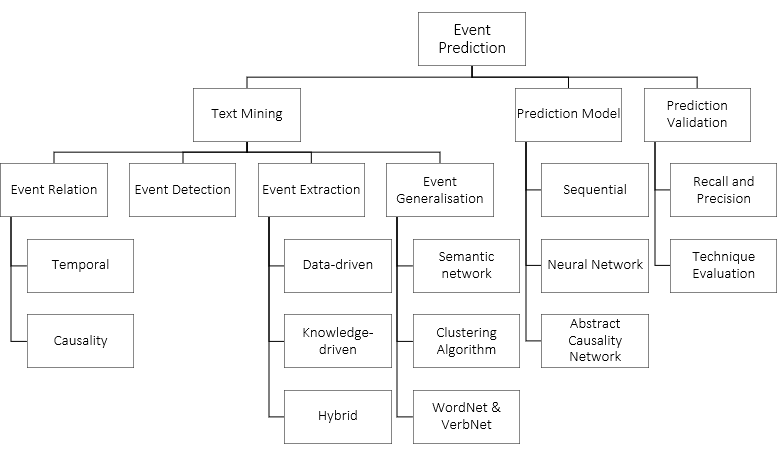
\includegraphics[width=1\textwidth]{./diagram/taxonomy}}
\caption{Taxonomy of Event Prediction - Generic steps needed to performed in event prediction}
\end{figure}  
\vspace{-1cm}
 
Event prediction involves in many domains. Research on areas of event prediction are active and wide. Example of domains in event prediction are below:
\begin{enumerate}
	\item Natural disaster such as earthquake \citep{asencio2017medium,asim2017earthquake} and tsunami \citep{mulia2016real},
	\item Political such as election prediction \citep{tung2016mining}
	\item Social such as protest event in Argentina  \citep{ning2016modeling}
	\item Economics such as predicting market stock price \citep{ding2015deep,vargas2017deep}, etc.  
\end{enumerate}

In news articles, there are many events happen everyday. From political issues, to social problems, economic trend and entertainments, newspaper provides public daily updates on these events. Recently, conflict happened on South China Sea (SCS) has becoming popular and continuously escalated. The happening of SCS conflict concerns countries nearby the regions and it must be solved and actions should be taken to prevent happening of any tragedy.     


\section{South China Sea Conflict}
South China Sea (SCS) is located strategically within Asia countries such as China, Taiwan, Indonesia, Philippines, Vietnam, and Malaysia. It has the busiest shipping lane as one-third of world's shipping passes through SCS and almost 3.37 trillion global trade happened within SCS in year 2016  \citep{chinapower2016}. Due to these huge market profit, many countries started to claim that SCS is their own territory and China even illustrated a "nine-dash line" which is a huge part from SCS and claim that region within "nine-dash line" is China's territory \citep{liuzhen2014}. These started the dispute between countries. For every dispute, public are able to know the flow of events through newspaper.

Examples of famous SCS dispute are Spratly islands dispute and China-Vietnam Military Clash. Spratly islands covered with huge amount of natural resources, global maritime areas and commercial shipping lane. In year 2015, China had militarised Fiery Cross Reef, reef located at the western edge of SCS and centre of Spratly islands by constructing military-level airstrip and seaport. This made concerns to Vietnam and Philippines as they felt threaten to their sovereignty in SCS region. Besides, China and Vietnam are continuously declared their ownership in SCS on oil and gas exploration issues. The issues are escalating as reports \citep{vietnamBoat2014} showed that Vietnam tried to ram Chinese vessels in SCS dispute area.     
 
New articles are written by different news agency with different perspective and opinion.Among many of the newspaper agency, National news agency such as Xinhua News Agency for China and Vietnam New Agency (VNA) are said to be the voice of government. \cite{gautierbattistellaOctober2005} stated that Xinhua is the biggest propaganda machine that spread the core concept of China's government to the public. Hence, there are huge amounts of valuable information that represent and reflect the action of government can be obtained within  news article from national news agency. However, without proper technique to extract useful information from the news article, the data source will be difficult to be obtained and time-wasting. In the next section, text mining will be introduced as an effective method to obtain valuable information from the news articles.   


\section{Text Mining}
Text mining, also known as knowledge discovery from textual databases and related with steps of obtaining valuable and non-trivial pattern or knowledge from unstructured text documents \citep{tan1999text}. A general framework proposed by \cite{tan1999text} in Figure 2.2 shows text mining contain two major elements, which are text refining and knowledge distillation. Text refining are techniques to transforms free-form text into intermediate form meanwhile knowledge distillation is to obtain the pattern or knowledges within the intermediate form. From text refining, two types of intermediate form can be obtained, document-based or concept-based which are able to be further processing into visualisation or predictive modelling.   

\begin{figure}[h]
\centering
\fbox{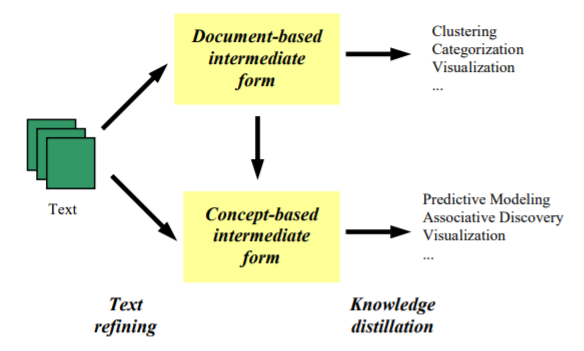
\includegraphics[width=1\textwidth]{./diagram/textMining}}
\caption{General Text Mining Framework proposed by \cite{tan1999text}}
\end{figure}

However, there are open problems in text mining that need be addressed. For examples, variety of intermediate form that causes complexity and uncertainty in text mining, multilingual text refining, domain knowledge integration \citep{lima2009domain}, and customized autonomous mining \citep{afzal2010rule}.

\subsection{Types of Data}
With text mining, useful information can be extracted for further processing. However, the volume of data is dramatically increasing nowadays, associated with high flow of data and high variety of information. For example, inside a single webpage, different type of data such as images, audio, textual data, comments, etc. can be obtained and categorised. Two major categories of data are structured data and unstructured data. Both of the categories will be further discussed in the following sections. 

\subsubsection{Structured Data}
Structured data is referred to the data that organisation all the information in formatted way and easily to extract and analysis by relational databases\citep{christinetaylor2018}. Example of structured data are phone number, name, identification numbers, date,etc. Format of structured data is analysable with human-generated queries and algorithm.  

\subsubsection{Unstructured Data}
Unstructured data is referred to the information that does not have a pre-defined model or structure and unable to store in traditional relational databases. Example of unstructured data such as text, emails, blogs, web pages, images, audio, comments on social media, etc. has no proper structure and has to be processing into valuable information before analysing them. Figure 2.3 shows the example of structure data(numerical and statistical data) and unstructured data(text, audio, video and blog posts).
\begin{figure}[H]
	\centering
	\fbox{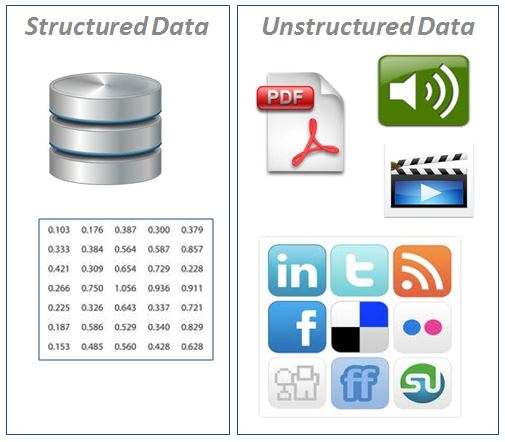
\includegraphics[width=0.7\linewidth]{diagram/Unstructured-Data-Examples}}
	\caption{Example of structured and unstructured data \citep{michaelbenzmoritzmuller}}
	\label{fig:unstructured-data-examples}
\end{figure}
\vspace{-1.5cm}

Nowadays, unstructured data is getting enormous. Information contained within these unstructured data originating from humans is absolutely richer and more valuable than traditional numeric data sources \citep{FRUNZA2016263}. Besides, study in 2019 \citep{rohitbigdata2019} showed that 95 percent of businesses need to manage unstructured data and more than 150 zettabytes(150 trillion gigabytes) of data will be needed for analysis by 2025. Because of that, exploring and extracting useful information from these unstructured data is essential. However, text mining is difficult due to ambiguity of languages, multiple duplicated words with different meanings, abbreviation, linked references etc\citep{bhardwaj2016text}.To overcome the difficulties, many techniques such as Named Entity Recognition (NER), Nature Language Processing (NLP), sentiment analysis, causality relationship extraction etc. are developed to extract high quality information from textual data. 

News event from SCS conflict is one of the unstructured data which the textual data is raw and does not have a proper structure on the sentences. Hence, further processing for the news events is important and it should be started with text preprocessing. 

\subsection{Event Relation}
Event relation is important in text mining as it provides better insight and understanding about event happens either before or after. Generally, there are 2 major type of event relation that can be observed and obtain from news article which are temporal relation and causality relation. As events happen from time-to-time, temporal attribute should be focused as it measures the trend and evolution of event. Besides, there is always a cause for events to happen, hence causality is used to relate events from the very beginning based on its cause.

\subsubsection{Temporal Relation}
Temporal is indicated as time-based or using time as the main measurement. Usually, events getting worse from a small case. For example, in medical domain, long-term follow-up is important for medical investigation. \cite{maziarz2017longitudinal} make use of temporal relation to observe the trend of patient's health condition over time, and eventually predict patients' risks for a future adverse outcome. Besides, temporal relation had been widely adopted in event prediction with different domain such as micro-blog and tweets \citep{preethi2015temporal}, sports \citep{grolinger2016energy}, stock market flow \citep{ding2015deep} and etc. 

\subsubsection{Causality Relation}
The main concept of causality is that one or more things/events as causes can cause one or more things/events to happen as effect. In news article, there are many events that related with each other but hard to be observe and detect by human or massive news events happen in the same time cause human hard to digest all the news happened in one time. Thus, people tend to automated the extraction of news article based on causality. However, there are many challenges in automating the process. For example, \cite{pechsiri2010explanation} faced difficulties on explanation knowledge graph through causality extraction from text such as causal-boundary determination and effect-event pattern determination. Nevertheless, it is useful for event extraction because it contain cause and effect that allows people to understand more about the following events. In this study, we will focus on causality relation as SCS conflict happens after certain small case instead of following time flow.  

\begin{enumerate}
	\item \textbf{Causality Pair}
	
	Causality pair is also known as entity pair, used to represent causality within pairs. For instance, \cite{mirza2014extracting} stated possible causality pairs in his study as (1) main events of consecutive sentences, (2) pairs of events in the same sentence, (3) an event and a time expression in the same sentence. If the pairs are tagged as (\textit{e\textsubscript{1},e\textsubscript{2}}), the pairs will be \textit{events-events}, \textit{events-timex}, \textit{timex-timex}. 
	
	\item \textbf{Causality Rules}
	
	After identify the potential cause-effect pairs, it is difficult to execute human-annotation on these causality pairs as the amount of data is getting enormous. Hence, autonomous annotation is proposed. 	In the work of \cite{radinsky2012learning}, Radinsky use causality rule to predict the future event as abstraction tree (AT) had been build earlier and using causality rules, a causality graph is built to explain the predicted event clearer.
	
	Moreover, in order to get an accurate categorised result based on causality pair, causality rules is set in every text extraction. \cite{zhao2017constructing} construct a set of causality rules that follows the template of <\textbf{Pattern,Constraint,Priority}> where Pattern indicates the trend of events between causality pairs, Constraint indicates the limitation on sentence which the pattern can be applied, Priority indicates the priority of causality pairs to be execute first or second. After extracting causality pairs from news article as well as generalise for more general purpose, an abstract causality network is built. 
		
\end{enumerate}

\subsection{Event Detection}
Event detection is a techniques to discover occurrences of events by analysing text stream in the sources. Generally, event detection can be broadly categorised as either Feature-pivot (FP) or Document-pivot (DP) \citep{fedoryszak2019real}. Based on \cite{chen2019bibliometric}, feature-pivot is the method that detecting abnormal patterns in appearance of features such as words. When an event happens, the frequency of a feature will be abnormal comparing to its unusual behaviour which indicating a potential new event. Meanwhile, document-pivot is using documents as items to clustered them by using similarity measure. 

The main idea of feature-pivot event detection is to represent the events as number of features that showing an abnormality in appearance counts.It is illustrated in Figure 2.4. These method rely on large amounts of dataset as the unusual frequency will be taken as important features.This technique is widely used in many domains especially in news documents. For example, \cite{mele2019event} use this technique to first extracts event features in tweets as well as clusters the documents according to the features. By finding a frequent pattern based on an infinite-state automation, it helps to model the changes in word frequency, state transitions as well as the events. This technique will also used in this project as Causality Mention (CM). By referring causality connector such as "because', "because of", "lead to" and "after" from \cite{zhao2017constructing}, the sentences that tagged with these connectors are selected and initially identified as event. 

\begin{figure}[H]
	\centering
	\fbox{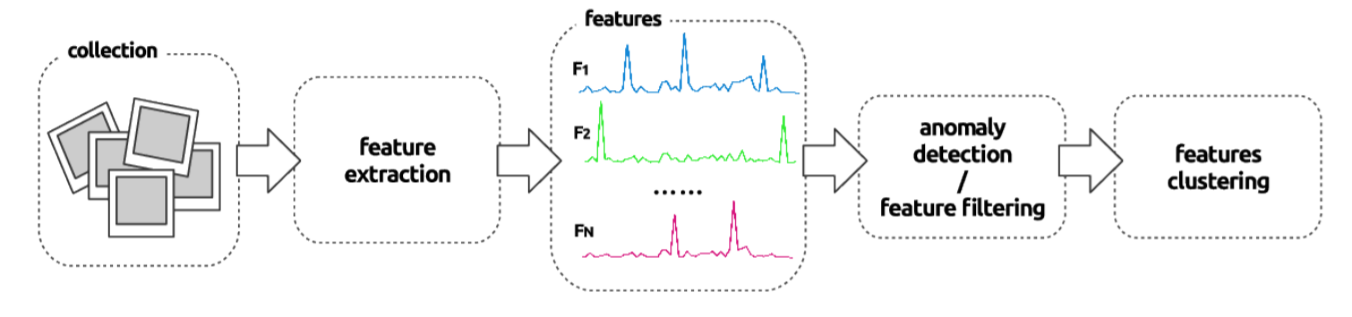
\includegraphics[width=0.9\linewidth]{diagram/feature_pivot}}
	\caption{Feature-pivot paradigm for event detection, adopted from \cite{schinas2018event}}
	\label{fig:featurepivot}
\end{figure}
\vspace{-1.5cm}

Document-pivot is a method where cluster documents based on their semantic similarity and group them into events. It is illustrated in Figure 2.5 This method is a bit different from traditional Bag-of-Words approach as it helps to identify event-related data that mixed with noisy data apart from clean data. TwitterStand \citep{sankaranarayanan2009twitterstand} is a news processing system using document-pivot approach to capture tweets corresponding to breaking news. However, this approach as low performance due to fragmentation of news topics, noisy content and the limited power of Bag-of-Words in short texts as tweets.  

\begin{figure}[H]
	\centering
	\fbox{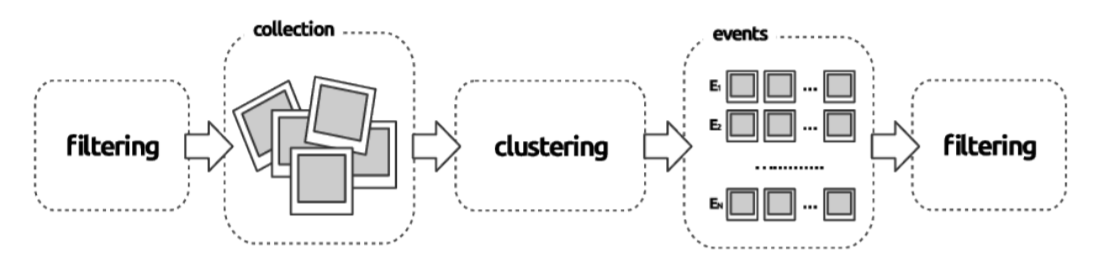
\includegraphics[width=0.9\linewidth]{diagram/document_pivot}}
	\caption{Document-pivot event detection, adopted from \cite{schinas2018event}}
	\label{fig:documentpivot}
\end{figure}
\vspace{-1.5cm}


\subsection{Event Extraction}
Event extraction is one of the common application of text mining as it obtains specific knowledge concerning incidents referred to texts \citep{hogenboom2011overview}.  Figure 2.6 shows the general procedure of event extraction. Event extraction uses data that are preprocessed using the methods mentioned in the previous chapter, and further represent by general causality pairs. 

\begin{figure}[H]
	\centering
	\fbox{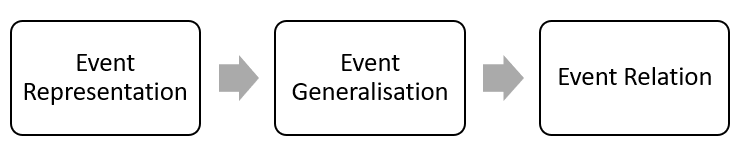
\includegraphics[width=0.7\linewidth]{diagram/eventRepresentation}}
	\caption{General procedure of event extraction}
	\label{fig:eventrepresentation}
\end{figure}
\vspace{-1.5cm}

Based on \cite{xiang2019survey}, event extraction is defined as one of the most important and active research domain in Naturral Language Processing. The author break down this big domain with several representative methods such as Pattern-matching, Machine Learning and also Annotation based on Cause and Effect. The following subsection will further discuss the concept and techniques' solution approaches. 

\subsubsection{Pattern-Matching}
Pattern-matching is a traditional event extraction method and require a specific template or structure to extract important information from the corpus. In order to obtain important insight from unstructured text, linguistic pattern is used to automatically build up a event patterns within the corpus. Figure 2.7 shows 13 linguistic patterns and example that applied to extract important information from corpus. For example, if given the a sentence, "victim was murdered". Based on the first linguistic pattern, "victim" will be tagged as <subject> while "murdered" will be tagged as verb. 

Figure 2.8 illustrate the process of event extraction based on pattern-matching. By following the linguistic pattern template, the sentence "They took 2-year-old Gilberto Molasco, son of Patricio Rodrigues" will be extracted with "took" as the trigger of the whole sentence and "Gilberto Molasco" as the subject or victim. Pattern-matching is domain-specific and works well in specific dataset. However, it does not provide accurate extraction in unstructured data such as news article and post in social media. 

\begin{figure}[H]
	\centering
	\fbox{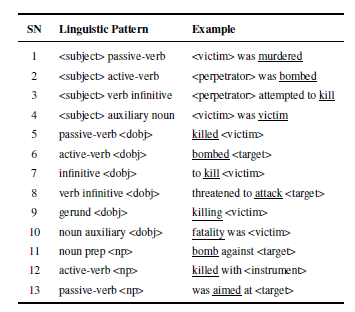
\includegraphics[width=0.8\linewidth]{diagram/linguisticPattern}}
	\caption{Example of Linguistic pattern and its pattern, adopted from \cite{riloff1993automatically}}
	\label{fig:linguisticpattern}
\end{figure}
\vspace{-1.5cm}

\begin{figure}[H]
	\centering
	\fbox{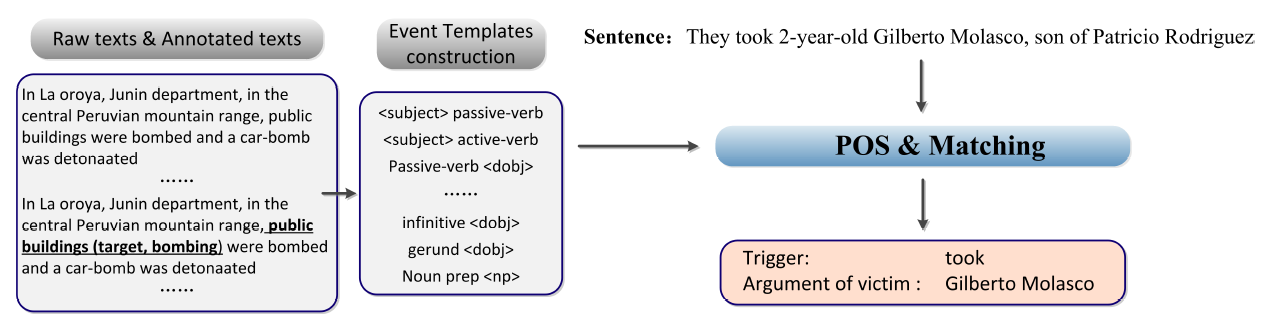
\includegraphics[width=1\linewidth]{diagram/patternMatching}}
	\caption{Example of event pattern construction and event extraction based on pattern matching adopted from \cite{xiang2019survey}}
	\label{fig:patternmatching}
\end{figure}
\vspace{-1.5cm}


\subsubsection{Machine Learning}
The important difference between pattern-matching based and machine learning based event extraction is that machine learning based event extraction rely on algorithm such as Support vector Machine (SVM), K-means clustering, etc. for the extraction. Apart of defining lingustic pattern, machine learning based event extraction learns classifier from training data based on feature engineering work. Feature engineering is a technique about creating new input features based on the existing one. In natural language processing, most of the comoon features can be divided as 3 types, \textit{lexical}, \textit{syntactic} and \textit{semantic} features. 

Lexical feature usually includes word lowercase and stopword removal, text lemmatization, Part-of-Speech (POS) tagging while syntactic features are extracted based on dependency parsing. The general idea of dependency parsing is to create edges between words in a sentences that denoting different types of relations. For example, Universal Dependencies \citep{deuniversal} documented standard dependencies for cross-linguistic typology such as nsubj, nmod, obj, etc. Figure 2.9 shows the example of dependency parsing on simple sentence, "Ivan is the best dancer". From this sentence, "dancer" is the root word and "Ivan" is the nominal subject (nsubj) to "dancer". Nominal subject is a noun phrase which is the syntactic subject of a clause. Besides, copula (cop) is the relation between verb and verb, determiner (det) is the relation between head of noun phrase and determiner and adjectival modifier (amod) is a adjectival phrase that represent the meaning of noun phrase. The representation helps to describe the grammatical relationship in a sentence so that researcher can understand more on the sentence. Lastly, semantic feature is normally includes obtaining synonyms of words as well as argument identification.

Figure 2.10 illustrate a overview of event extraction based on machine learning approach. From the figure, each of the features are embed into vector which is also another important concept that will be discussed on the following subsection. 

\begin{figure}[H]
	\centering
	\fbox{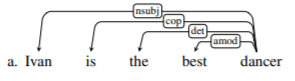
\includegraphics[width=0.8\linewidth]{diagram/dependencyParsing}}
	\caption{Example of Dependency Parsing Visualisation}
	\label{fig:dependencyparsing}
\end{figure}
\vspace{-1.5cm}

\begin{figure}[H]
	\centering
	\fbox{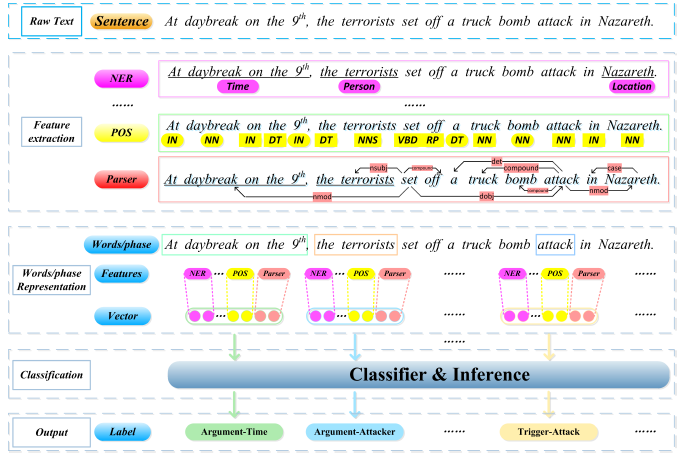
\includegraphics[width=1\linewidth]{diagram/extraction_machineLearning}}
	\caption{Example of event extraction based on machine learning}
	\label{fig:extractionmachinelearning}
\end{figure}
\vspace{-1.5cm}


\subsubsection{Cause-Effect Annotation}
Annotation is an important concept in obtaining useful information in Natural Language Processing (NLP). By annotating raw text data, all the text become meaningful as tag with specific characteristics. For example, a Named Entity Recognition (NER) annotation can simply help researchers to eliminate most of the noise in the raw data by only obtaining Person, Location, Time, etc. The most widely used annotation tools for NLP is Brat and WebAnno. Figure 2.11 shows the screenshot of Brat annotation tools. By using Brat, cause and effect can be easily annotated followed by their relationship (cause-effect). 

One of the well-known test data for cause-effect annotation is SemEval-2010 Task 8 \cite{hendrickx-etal-2010-semeval}. It is a standard test data for multi-way classification of semantic relations between pairs of nominals. In this dataset, there are many semantic relations annotated such as Cause-Effect (CE), Instrument-Agency (IA), Product-Producer (PP), etc. In this research, CE will be focused and the extracted cause and effect will be taken as test data for model validation. 

\begin{figure}[H]
	\centering
	\fbox{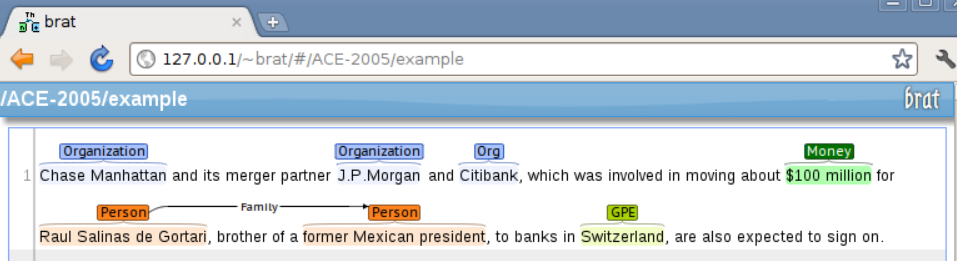
\includegraphics[width=0.7\linewidth]{diagram/bratAnnotation}}
	\caption{Screenshot of Brat Annotation Tool}
	\label{fig:bratannotation}
\end{figure}
\vspace{-1.5cm}
 
Table 2.1 shows the recent research for event extraction as well as their approach and limitation. Most of the research is based on machine learning approach since it provides a feed forward neural network for continuous word or sentence representation. It might be helpful in dealing with large raw text corpus and highly unstructured data. 
 
\begin{table}[H]
\fontsize{11}{12}\selectfont
\caption{Comparison of Recent Research on Event Extraction}
\renewcommand{\arraystretch}{1}
\begin{tabular}{|p{2cm} |p{4cm} |p{2cm}|p{5cm}|}
	\hline 
	Author, year & Domain & Approach & Limitation \\ 
	\hline 
	\citep{valenzuela2015domain}&Domain-independent Rule-based Framework for Event Extraction  & Pattern-Matching & Needs to design multiple rules for different domain  \\ 
	\hline 
	\citep{ritter2012open}&Open domain event extraction from twitter  & Machine Learning & Segmentation error on unknown words on Tweet  \\ 
	\hline
	\citep{wu2017event}&Event Timeline Extraction on News Corpus & Machine Learning  & Require large text corpus \\ 
	\hline 
	\citep{vossen2016newsreader}&Using knowledge resources in cross-lingual reading machine from news  & Machine Learning & Require knowledge acquisition and NLP improvement on a massive scale \\ 
	\hline 
	\citep{rospocher2016building}& Building event-centric knowledge graphs from news & Annotation & Expert knowledge required to build knowledge graph \\ 
	\hline 
	
\end{tabular} 
\end{table}
\vspace{-1cm}

\subsection{Event Representation}
Event from news article usually construct based on sentences or phrases. However, unstructured raw text is highly ambiguous and without proper rules or structure, machine wouldn't know any meaning from these text. \citep{mikolov2013distributed} proposed a method called distributed representation of words in vector space or word embedding that actually helps natural language processing to achieve better performance in term of linguistic understanding. These word embedding approach is useful in term of capturing semantic and syntactic patterns between words. Below are some example of state-of-art word embedding technique: 

\subsubsection{Word Embedding}
In word embedding, the most commonly used technique is Latent Semantic Analysis (LSA), Word2Vec and Glohal Vector (GloVe). 

\begin{enumerate}
	\item \textbf{Latent Semantic Analysis (LSA)}
	
	LSA is a statistical technique by using bag-of-words where it convert every words in document into vector by counting the number of occurrences of each words in the documents. Then, a term-document matrix (TDM) is constructed for the document vectors. The core concept of LSA is term frequency where it take weighting scheme (boolean of O-term not used and 1-term is used) into consideration. Figure 2.12 shows an illustration of TDM and a singular value decomposition is used to get the most closest vector embedding in the subspace. 
	
	\begin{figure}[H]
		\centering
		\fbox{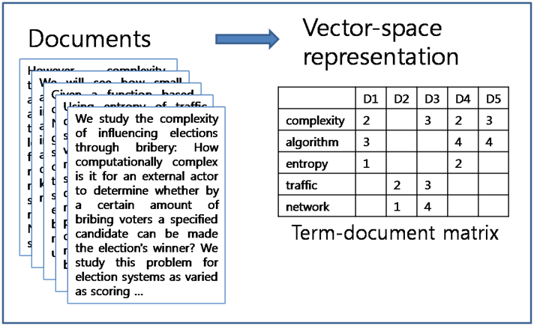
\includegraphics[width=0.7\linewidth]{diagram/term_document_matrix}}
		\caption{Term-document Matrix}
		\label{fig:termdocumentmatrix}
	\end{figure}
	
	\item \textbf{Word2Vec}
	
	Word2Vec is first proposed by \cite{mikolov2013distributed} as a solution for neural network based training of word embedding. Until now, Word2Vec is becoming the state-of-art word embedding algorithm as many of the research extends from this concept such as \cite{zhang2015chinese}, \cite{lilleberg2015support}, etc. 
	
	There are 2 different approaches in Word2Vec, Continuous Bag-of-Words (CBOW) and Skip-gram model. Figure 2.13 shows illustration of CBOW and Skip-gram in Word2Vec. CBOW is trained and learning to predict the word by context as well as maximize the probability of the target word by finding the context. For example, given a context "yesterday was a really [...] day". CBOW model will be about to predict the possible target word as "beautiful" or "nice". On the other hand, skip-gram model is a reverted version of CBOW as it is used to predict the context. Given a word "beautiful", there are higher possibilities that "yesterday was really [...] day" will be selected as the context.
	
	The most common downstream application that applied Word2Vec algorithm is smartphone keyboard. Word2Vec helps to implement next-word prediction feature to ease smartphone user during their text typing. Besides, Word2Vec also helps in getting valuable information from customer reviews. Business can use this technique to analyze survey responses and perform business analytic on these data.  
	
	\begin{figure}[H]
		\centering
		\fbox{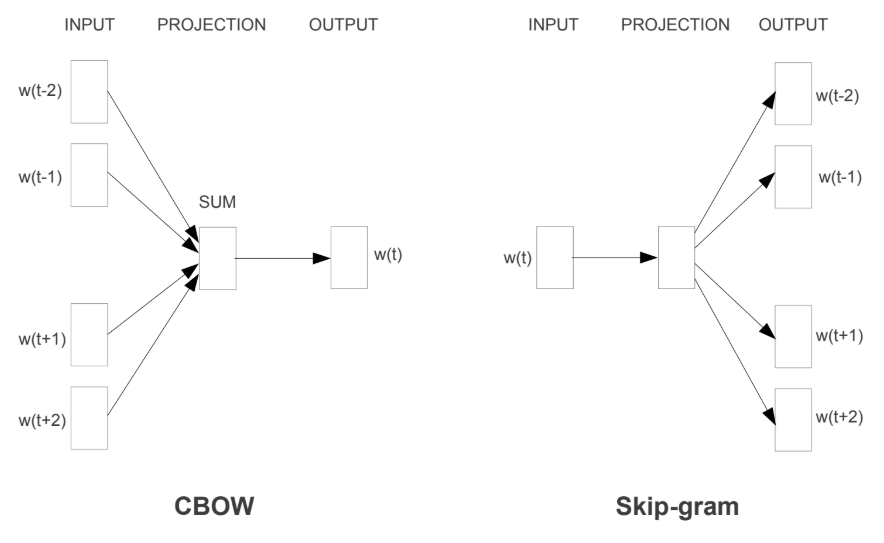
\includegraphics[width=0.7\linewidth]{diagram/word2vec}}
		\caption{Word2Vec training model, adopted from \cite{mikolov2013efficient}}
		\label{fig:word2vec}
	\end{figure}
	
	
	\item \textbf{Global Vector (GloVe)}
	
	GloVe stands for Global Vector for Word Representation. It was proposed by  \cite{pennington2014glove} and soon become one of the state-of-art word embedding model due to its faster training speed by using non-zero matrix entries. GloVe is training on word co-occurrence matrix and its probability and ratio between target words and context words from 6 billion token corpus. Besides, GloVe provides a pre-trained word vectors for different domains such as Wikipedia, Common Crawl and also Twitter. All of the pre-trained model will be trained in different vector dimension to fix the usage of researchers. In this research, GloVe pre-trained word vectors will be one of the reliable resource in loading word vectors since training word vector from scratch is time-consuming and relatively expansive in computational resource. 
	
\end{enumerate} 

However, word embedding seems not sufficient when it comes to phrase or sentence level. For phrase or sentence level embedding, most of the approach will be simply averaging a sentence's word vector/ Bag-of-words approach. This brings to several constraint in word embedding such as semantic similarity between sentences. word embedding only consider to represent the meaning of 1 word into vector and when comes to phrase and sentence, it cannot represent accurately the meaning of phrase or sentence. To address this problem, sentence embedding technique is used. The following subsection will discuss several sentence embedding technique such as Doc2Vec, InferSent and BERT.    

\subsubsection{Sentence Embedding}

\begin{enumerate}
	\item \textbf{Doc2Vec}
	
	Doc2Vec is proposed by \citep{le2014distributed}. It is also known as Paragraph Vector as the algorithm added a Paragraph ID on its training. Based on Word2Vec approach, Doc2Vec follows the concept of CBOW and skip-gram, additionally added another vector (Paragraph ID). There are also 2 method that similar to CBOW and skip-gram in Word2Vec which are PV-DM (Paragraph Vector - Distributed Memory) and PV-DBOW (Paragraph Vector - Bag-of-Words). Figure 2.14 shows the illustration of PV-DM and PV-DBOW model. PV-DM predict the missing target word in the context while PV-DBOW predict all the context from the target word. 
	
	\begin{figure}[H]
		\centering
		\fbox{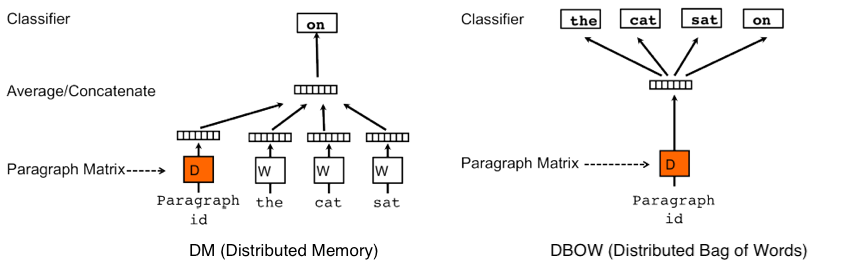
\includegraphics[width=0.8\linewidth]{diagram/doc2vec}}
		\caption{PV-DM and PV-DBOW model in Doc2Vec \citep{le2014distributed}}
		\label{fig:doc2vec}
	\end{figure}

	Doc2Vec is a unsupervised learning algorithm that learns vector representation for variable-length pieces of texts. Doc2Vec had achieved good performance compared with other baseline sentence vector embedding. From Figure 2.15, Doc2Vec achieved lower error rate of 3.82\% compared to other baseline method. Hence, Doc2Vec is one of the sentence embedding technique will be used in this research.                             
	
	\begin{figure}[H]
		\centering
		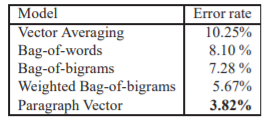
\includegraphics[width=0.8\linewidth]{diagram/doc2vec_performance}
		\caption{Performance of Paragraph Vector (Doc2Vec) and other baseline on information retrieval task \citep{le2014distributed}}
		\label{fig:doc2vecperformance}
	\end{figure}
	
		
	\item \textbf{InferSent}
	
	InferSent is a one of the state-of-art sentence embeddings method that provides semantic sentence representation. Facebook researcher had proposed InterSent in this paper \cite{conneau2017supervised}. Figure 2.16 shows the simplified illustration of how InferSent works. InferSent first embed the sentence using sentence encoder. There are several technique in the sentence encoder and one of the most effective technique is Bi-directional LSTM network with max or mean pooling. Each vector is concatenate between forward LSTM and a backward LSTM that able to read sentence in opposite direction. Then, max or mean pooling is used in these concatenated vector to form fixed-length vector.  
	
	
	Natural Language Inference (NLI) or textual entailments is a method of finding directional relationship between text fragment. InferSent make use of Stanford Natural Language Inference (SNLI) dataset and manually labelled with 3 categories (entailment, contradiction and neural), then create NLI classifier. NLI classifier is then used to extract the relations between text and hypothesis. 
	
	\begin{figure}[H]
		\centering
		\fbox{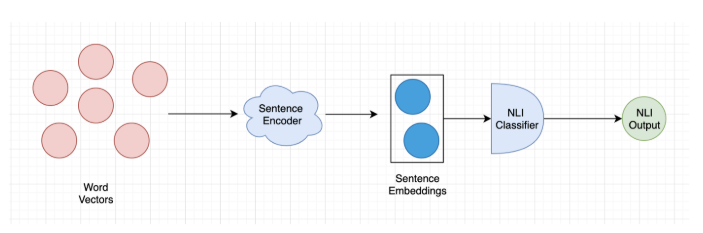
\includegraphics[width=0.8\linewidth]{diagram/infersent}}
		\caption{Simplified Illustration of InterSent}
		\label{fig:infersent}
	\end{figure}

	Due to InferSent's semantic representation, this research will be using InferSent as one of the sentence representation method to be compared with both Doc2Vec and BERT. 
	 
	
	\item \textbf{BERT} 
	
	BERT stands for Bidirection Encoder Representation from Transformers is a state-of-art sentence embedding technique proposed by Google AI language. \citep{devlin2018bert}. BERT make use of Transformer, an attention mechanism that learns contextual relation between words in a text. 
	
	Figure 2.17 shows the BERT input representation. There are 2 important element in BERT, Masked LM (MLM) and Next Sentence Prediction (NSP). MLM allows bidirectional training where the model uses the context words surrounding a [MASK] token and try to predict what the [MASK] word should be. Besides, in NSP, [CLS] token is inserted at the beginning of first sentence while [SEP] token is insert at the end of each sentence. Combining with [MASK] token, it forms a sequence and the entire sequence will be embeded through Transformer model.
	
	Due to the bi-directional representation behaviour and transformer encoder in BERT, BERT have a highest accuracy in Semantic Text Similarity (STS) score. It obtain the highest (86.5\%) similarity score compared to other sentence embedding algorithm such as Pre-OpenAI SOTA (81.0\%), BiLSTM+ELmo+Attn (73.3\%) and OpenAI GPT (80.0\%) \citep{devlin2018bert}. Hence, in this research, BERT will be used as one of the sentence embedding method for measuring text semantic similarity
	
	\begin{figure}[H]
		\centering
		\fbox{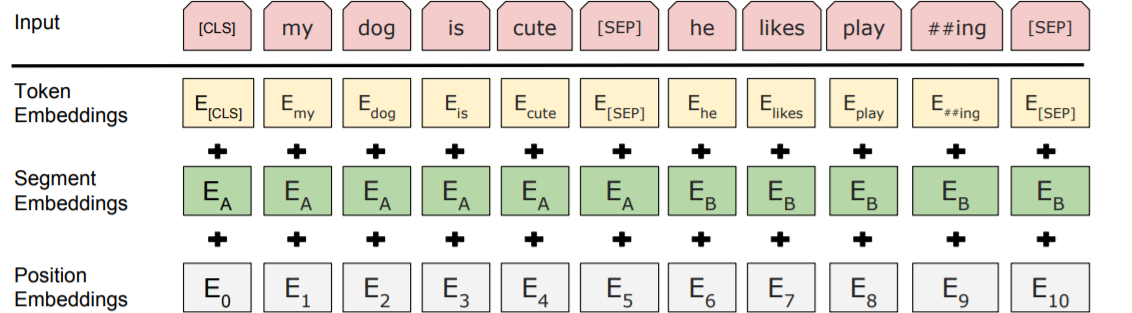
\includegraphics[width=0.9\linewidth]{diagram/bert}}
		\caption{BERT input representation \citep{devlin2018bert}}
		\label{fig:bert}
	\end{figure}
	
	
	
\end{enumerate}


\section{Prediction Model Technique}
Prediction model technique is an algorithm that modelling prediction and provides a guideline throughout the process of building up a predictive model. After obtaining extract keyword from textual data and clustering them based on clustering algorithm and relation extraction, the data is now said to be clean and sanitised. These clean data is then involve in prediction algorithm to build up a prediction model.
 
\subsection{Sequential Prediction Algorithm}
Sequential prediction is a fast and simple pattern matching algorithm whereby comparing the past data or experience on a linear running timeline. There are many examples for sequential prediction algorithm such as medical condition that occur over time and patient conditions is getting either better or worse based on previous event. Besides, suggestion system that used in music application such as Spotify also involve in sequential prediction. 

\subsection{Neural Network Prediction Algorithm}
The biggest advantages of applying neural network in event prediction is the high tolerance and acceptance ability of noisy data and high accuracy. Despite of its complexity and long training time, many researches are more towards to neural network.\citep{granroth2016happens,hu2017happens,asencio2017medium} Neural network use the concept of brain metaphor for information processing and is suitable to discover previously unknown, valid patterns and relationship in large data sets. \citep{gaur2012neural}

\subsection{Vector Similarity}
Vector similarity is one of the important measure for word vector or sentence vector. Example of technique measuring vector similarity are Cosine Similarity, Euclidean distance, Jaccard distance and word mover's distance. Among these techniques, Cosine similarity is being widely used in applied in NLP domain. \citep{torabi-asr-etal-2018-querying, mikolov2013distributed, bekkali2019effective}. Equation 2.1 shows the formula of cosine similarity.

\begin{equation}
\frac{A.B}{||A|| * ||B||}
\end{equation}

Cosine similarity is used for chat bot engine \citep{yang2018learning}. When user input a random query, the input will be embed into vector and compute cosine similarity calculation with every vector in the model. After that, vector with highest similarity will be selected and returning the original question. The question is said to have the most similar textual semantic to the input query. This question is then linked user to the coresponding answer. 

In this research, cosine similarity is one of the most important element to be calculated so that similarity between sentence can be measured for accurate result.   




\section{Existing work of Event Prediction}

\begin{table}[]
	\vspace{-1cm}
	\centering
	\caption{Existing work on Event Prediction}
	\renewcommand{\arraystretch}{1.2}
	\noindent\makebox[\textwidth]{
		\begin{tabular}{|p{3cm}|p{3cm}|p{5cm}|p{4cm}|}
			\hline
			\textbf{Author, year} & \textbf{Work}                                                                                                                    & \textbf{Method}                                                                                                                                                                                                                                                                                             & \textbf{Advantages/ Limitation}                                                                                                  \\ \hline
			\citep{letham2013sequential}& Sequential event prediction  & Given a sequence past database to predict next event within a current event sequence & Rely on additional user input, supervised ranking algorithm which not suitable for less predictive power past events \\
			\hline
			\citep{mirza2014extracting}   & Temporal sentiment analysis and causal rules extraction from tweets for event prediction & Event prediction based on temporal sentiment and causality from tweets which are from the opinion of people & Sentiment from tweets is uncertain and may affect on the predictive output \\
			\hline
			\citep{ding2015deep}  & Depp learning on event-driven stock market prediction  & Extract news text with dense vectors and train with novel neural tensor network, provides prediction based on convolutional neural network & Outcome is more focus on statistical, less focus on financial news that affect the share price in the market\\
			\hline
			\citep{hu2017happens}  & Event Prediction using Compositional Neural Network Model    & Use word2vec to represent events and build a compositional neural network model for future event prediction & Multiple event chain in CNN models and limited to learning associations between pairs of events \\
			\hline
			\citep{li2018constructing}   & Narrative event evolutionary graph (NEGG) for script event prediction  & Extract narrative event chain from newspaper and construct NEEG based on the chain &  Require expert knowledge in deep learning to produce NEGG   \\
			\hline
			\citep{rumi2018crime} & Crime event prediction with dynamic features and matrix factorisation   & Dynamic features such as visitor entropy, visitor homogeneity, region popularity, visitor ratio and count, observation frequency is taken as measurement in crime event prediction & Different city have different crime data, result may be biased \\
			\hline
			\citep{dami2018news}   & News events prediction using Markov logic networks & Markov logic network represent complex events by first-order logic and binded with domain-specific causal rules. Web ontology language (OWL) perform causal inference to represent probabilistic knowledge & Domain-specific causal rule must be created precisely before further text processing \\     
			\hline                                                                                                 
	\end{tabular}}
\end{table}

There are several researchers research on the topic 
of event prediction based on causality attributes and combining different method on different domain. Table 2.2 shows the existing work of event prediction, focusing on textual data from different domain such as financial, social media, medical etc. 

In the previous works, trend of event prediction starts from sequential approach, transforms to deep learning and even involved in neural network model. Researchers found that deep learning and neural network model able to cope with the high variety of unstructured textual data. Besides, event extraction also slowly transform from data-driven approach into knowledge-drive approach which able to observe from the latest work of \cite{dami2018news} that using Markov logic network with knowledge-driven extraction approach. In addition, among these previous study, causality is the main attribute that concern by the researchers. In this study, causality will also be the main attribute followed by different embedding technique. Besides, vector similarity will also be used to determine the semantic similarity between corpus embedding and input queries' embedding. Finally, the most similar cause in corpus will be taken and the linked effect will be taken as the possible predicted output.


\section{Open Issues and Challenges}
Event prediction is important and useful for public to have better insight and quick response against event might happen. However, there is several issues and challenges need to be addressed in order to produce a perfect predictive model approaching human-thinking. The issues and challenges are: 
\begin{enumerate}
	

\item \textbf{Low performance of predictive model due to low resource scenarios}

For predictive model, it require as much data as possible to train and test its accuracy and improve any weakness that learning from bad data sources. However, one of the problem is that there are scenarios of low resource that the prediction model can obtain. For example, if the model receive data source that are unique and only few events occurs because of these, the predicted output might not be valid and match with human-predicted output. 

\item \textbf{Word Sense Disambiguation}

In textual data extraction, word sense disambiguation is an open problem that troubling in determine the sense of word used in a sentence. One of the significant example can be observe in differences between dictionaries. 
For example, the word "\textbf{bank}" has 3 different meaning according to Cambridge Dictionary. First, bank is indicated as financial organisation where people can invest or store money inside, second is sloping raised land along sides of river, third is related to row of similar things. There are 2 sentences, "The \textbf{bank} will not be open in Saturdays" and "the river overflowed the \textbf{bank}.". The ambiguity between 2 same words but different meaning make machine difficult to detect and extract correct information from its true nature.

\item \textbf{Pronoun Resolution}

Pronoun resolution also known as anaphora resolution, is an common problem of resolving what a pronoun, or a noun phrase refers to. \citep{poesio2016anaphora}. Taking example of "John helped Mary", followed by "He was kind". As normal human, we can understand that "he" is indicating to John but not the machine. Machine will automatically define "he" as a new character instead of combining John with "he". Anaphora resolution is still an active research \citep{choi2016coreference,bandaragoda2018text} which contributes to better machine learning technique. 

\end{enumerate}
\section{Summary}
In this literature review, concept of event prediction and South China Sea conflict is clearly explained before moving in brief stage of event prediction. Then, stages within event prediction such as text mining, clustering, event relation extraction, prediction algorithm and etc is mentioned with details in the previous subchapter. Finally, this chapter discuss about previous and existing work that done by other researchers on the textual data event prediction in different domain and also the open issues and challenges in event prediction so that reader get better understanding about constraints of event prediction nowadays. 



% Chapter 3
\chapter{Research Methodology}

\section{Overview}
This study focuses on the implementation of vector similarity measure with different sentence embedding technique for event prediction on South China Sea conflict. In this research, causality relation will be focused. This chapter emphasises the research framework of the study which explains the method and technique used to achieve the objective of the study. This chapter begins with the overview of research framework which consists of three phases and each phase will be briefly explained. Besides, overall research plan will be provided in order to give a better understanding on overall expected result of this study. After that, the chapter continues with brief description of data set which will be used in this study. Finally, the chapter ends with summary. 

\section{Research Framework}
\begin{figure}[H]
	\centering
	\includegraphics[width=1.0\linewidth,height=0.9\textheight]{"diagram/Research Framework"}
	\caption{Research Framework}
	\label{fig:research-framework2}
\end{figure}

The research framework consists of three phases which correspond to the three research objectives in Chapter 1. The three phases are; (i) Causality data corpus building based on South China Sea conflict news article, (ii) Phrase representation and phrase similarity measure, (iii) Causality prediction model. The flow of these three phases is illustrated on the research framework in Figure 3.1.

In phase 1, news event will be represented in <cause, effect> format where it is named as causality pairs. Data is collected from various online news article that concerned on South China Sea conflict within China and Vietnam. After data collection, the following steps is causality mention extraction. Causality mention extraction will use specific causality connector such as "because", "because of", "after", etc to extract sentences that contain causality event. After that, "cause" and "effect" sentence will be extracted based on the annotation in order to clearly identify "cause" and "effect" sentence. Finally, event is represented in the causality pairs format of <Cause, Effect>. 

In phase 2, phrase embedding model and phrase vector will be generated. 
<Cause, Effect> causality pairs from phase 1 are further extracted by using verb-and-noun representation. Verb-and-Noun representation is used because it preserve most of the important information rather then losing them. After extracting important information, the words is further generalised using WordNet and VerbNet. Each noun is generalised to its hypernym in WordNet while each verb is generalised to its class in VerbNet. Furthermore, frequently co-occurring word pairs (FCOPA) is used to identify the frequent term and will be represented as node of abstract causality network. The edges of causality network is constructed if there is existing edge in specific event. 

In phase 3, prediction model based on causality network embedding model will be proposed. Dual cause-effect transition (Dual-CET) model will be used for adopting essential characteristics of event causality such as asymmetry, transitivity and many-to-many. Besides, a ranking criterion will be used in order to learn the correct event embedding based on true causality pairs. Next, the Dual-CET model is measured by several evaluation criterion such as Random, Common neighbours, Jaccard's coefficient, etc to measure the effectiveness and reliability of the model.  
  
In addition, the main purpose of overall research plan is to provide a clear idea solve each research question that based on research objective, associated with its methodology and expected result.The overall research plan is tabulated in Table 3.1. In the first objective, the expected result should extracted keywords from South China Sea conflict-related news article in China and Vietnam as well as extract the causality connectors and represent them in causality pairs of <cause, effect> format. Meanwhile, in phase 2, the causality pairs will be further processed with causal event extraction and generalisation and visualise the causality network with nodes and edge based on processed causality pairs. Lastly, in phase 3, the study will focus on proposal of predictive model, which consist of building abstract causality network with frequently co-occurring word pairs (FCOPA) and embed the network with Dual-CET model. 

	\begin{table}[]
		\vspace{-1cm}
		\small
		\centering
		\caption{Overall Research Plan}
		\renewcommand{\arraystretch}{1.5}
		\noindent\makebox[\textwidth]{
	\begin{tabular}{|p{3cm}|p{3cm}|p{4cm}|p{4cm}|p{3cm}|}
		\hline 
		Research Objective & Research Question & Methodology & Result & Performance Measure \\ 
		\hline 
		To extract <cause, effect> causality pairs from news articles in South China Sea conflict by using causality connectors 
		& How to obtain useful information from news article that related to South China Sea conflict?  
		& 
		\begin{minipage}[t]{\linewidth}
			\begin{itemize}
				\item Build news article corpus of SCS conflict from online news article that focus on issues within China and Vietnam 
				\item Extract causality pairs of <cause, effect> using causality connectors based on template of <Pattern, Constraints, Priority> 
			\end{itemize} 
		\end{minipage}
		& 
		\begin{minipage}[t]{\linewidth}
				\begin{itemize}
				\item News article on South China Sea conflict within Vietnam and China is extracted and created news corpus.
				\item Event is extracted and represented in <cause, effect> causality pairs format. 
			\end{itemize} 
		\end{minipage}
	
		& Make sure event pairs is represented in <cause, effect> format \\ 
		\hline 
		To extract all important information from causality pairs by using verb-noun representation as well as discover general patterns using WordNet and VerbNet. 
		& How to generalise and cluster event extraction and how to relate event pairs with causality? 
		& 
	 	\begin{minipage}[t]{\linewidth}
 			\begin{itemize}
 			\item Extract all the important information within causality pairs by using verb-noun representation.
 			\item Generalise all the verb and noun with WordNet and VerbNet. 
 		\end{itemize} 
	 	\end{minipage}
		& 
		\begin{minipage}[t]{\linewidth}
		 \begin{itemize}
			\item All the important information will be kept while eliminating unused information.  
			\item All information is generalised to produce a general, frequent and simple causality patterns. 
		\end{itemize}
		\end{minipage}
		& Visualise causality network with nodes and edge \\ 
		\hline 
		Train and build an abstract causality network with frequently co-occurring word pairs (FCOPA) and embed the model into a continuous vector space. 
		&How to use the extracted information to train and build a prediction model?
		&
		\begin{minipage}[t]{\linewidth}
			\begin{itemize}
				\item Build abstract causality network with frequently co-occurring word paris (FCOPA)
				\item Embed causality network with Dual-CET model.
			\end{itemize}
		\end{minipage}
	 	& 
		\begin{minipage}[t]{\linewidth}
			\begin{itemize}
			\item Prediction model will be generated and able to generate general predicted output based on inputted event.
			\item Accuracy of prediction model is measured.  
			\end{itemize}
		\end{minipage}
	 	 & 
		Examine prediction model by performing several evaluation criterion such as Random, Common neighbours, Jaccard's coefficient.\\ 
		\hline 
	\end{tabular}} 
\end{table}


\subsection{Phase 1}
Phase 1 is causality data corpus building and it is important to convert unstructured data from news article to structure form and understandable by the computer. There are several steps to build up a good data corpus which involve specific data collection, causality mention extraction and event representation.
\begin{enumerate}[label=(\alph*)]
	\item Data Collection
	
	The data is collected from news article based on keyword of South China Sea conflict such as "South China Sea", "ASEAN", "Spratly", "Island", "People's Court",etc. In the news article that consist of these keywords, these articles are taken according to the country where the news being published. This will be further explains in the subsection of data set. 
	
	\item Causality Mention Extraction
	
	In causality mention extraction, the selected news article is then further selected with causality connectors such as "because", "because of", "after", "therefore", "lead to", etc. First of all, sentence segmentation will be used to split all of the sentence in the article. Then, all of the sentence is filtered by causality connectors. After that, regular expression (Regex) will be used to setup extraction rules and pattern and return the result of "cause" and "effect". 
	 
	\item Event Representation
	
	In event representation, causality pairs format will be used as each sentence is represented as \textit{<Cause, Effect>}. This representation can be done from obtaining the value based on the pattern of regular expression. For multiple data that obtained in multiple article, all the causality pairs is stored in JSON format. 
	
\end{enumerate}
\subsection{Phase 2}
Phase 2 is discussing about abstract causality network by using causal event extraction and generalisation. After obtaining causality pairs, the pairs still needed to be further processing in order to obtain useful information. At this stage, both cause and effect triple is now in sentence form. In order to obtain and preserve all the information within the triple, verb-and-noun representation is used. After that, all the verb and noun within the triple are generalised using WordNet and VerbNet. Then, the specific causality network is build by using these information. In order to obtain a frequent, general causality pattern, the causality pair is then generalised with frequently co-occurring word pairs (FCOPA) to build up abstract causality network. 

\begin{enumerate}[label=(\alph*)]
	\item Causal Event Extraction
	
	For shrinking down the causality pairs that obtained from the previous steps, causal event extraction is needed. First, POS tagging is used to tag out all the words with their unique characteristics. Then, for each verb, noun and proper noun will be taken and update the triple. Meanwhile, the remaining words will be removed. 
	
	\item Causal Event Generalisation
	
	After extraction, there are still a lot of redundant and similar words within the triple. Hence, generalisation is needed. By using WordNet, noun and proper noun will be generalise to their synonym or hypernym while verb will be generalised to its class by using VerbNet. 
	
	\item Abstract Causality Network
	
	After generalise all the event pairs, the event pairs is linked by using pyvis visualisation library. By using "cause" and "effect" as nodes and each event pair has the edge, build up an abstract causality network. Generalised nouns and verb may be redundant as it is perfect for the abstract causality network in term of diversity.  
	
	
\end{enumerate}
\subsection{Phase 3}
Phase 3 is to train and build a new embedding model, dual cause-effect transition (Dual-CET) model as the predictive model. 
In machine learning, a model that generated needs to be trained as the model will dynamically learn the pattern from the inputs and fix any error that occurred during its training. In this study, a new cause event will act as input and predicted effect events will act as output. While adding the input cause event into the model, steps need to be taken as guideline for the overall event prediction.  

\begin{enumerate}[label=(\alph*)]
	\item Dual-CET model 
	
	In this study, Dual-CET model is proposed by embedding abstract causality network that created in phase 2. By considering cause-to-effect and effect-to-cause possibilities, a new energy function, f(c,e) is defined, 
	\begin{equation}\label{3.2}
	f(c,e) = || c + t + e||_{1} + || e + \tau - c||_{1}
	\end{equation}where c and e are cause and effect, +t and +$\tau$ are the encoding of many-to-many, asymmetry and transitivity of event causality. 
	
	 

\end{enumerate}
\section{Data sets}
This study will focus on South China Sea conflict news article from online resource within China and Vietnam. Keywords such as "China", "Vietnam","South China Sea", "Spratly", "World Court" will be used to search online news article. Once the news article matched with the keywords, it is taken as our data sets for further data processing.The collected data is then grouped according to corresponding country based on the location of the news published. For example, if the news are published in Hanoi, the news is grouped into Vietnam since Hanoi is one of the state in Vietnam. In this study, only 30 online news from China news agency and 30 online news from Vietnam news agency will be taken. In Figure 3.2 and 3.3, sample of news article from Vietnam and China is taken from online resources and put into .txt document file.          
\begin{figure}[H]
	\centering
	\fbox{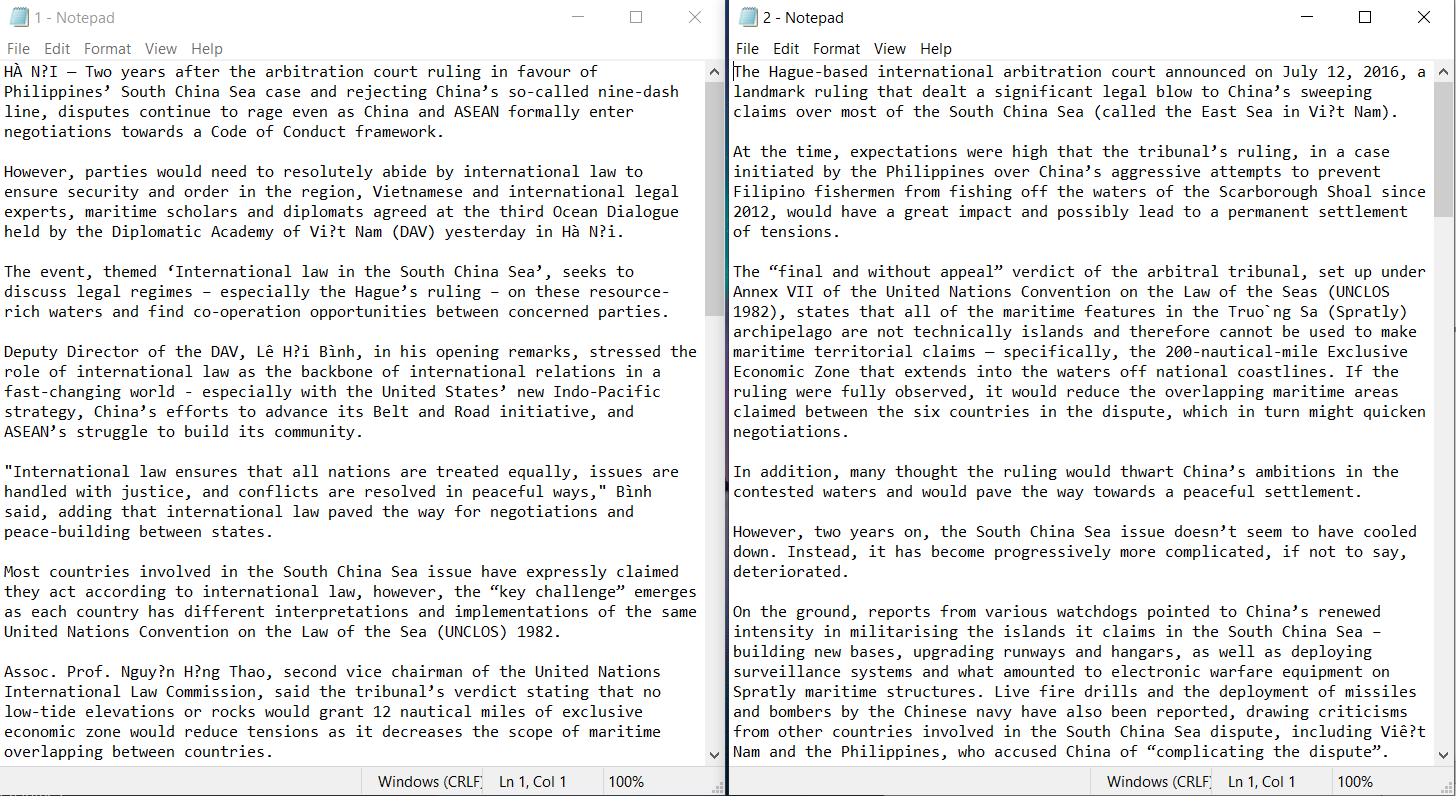
\includegraphics[width=1.0\linewidth]{diagram/vietnamNews}}
	\caption{Sample of news article from Vietnam New Agency}
	\label{fig:vietnamnews}
\end{figure}
\vspace{-1cm}
\begin{figure}[H]
	\centering
	\fbox{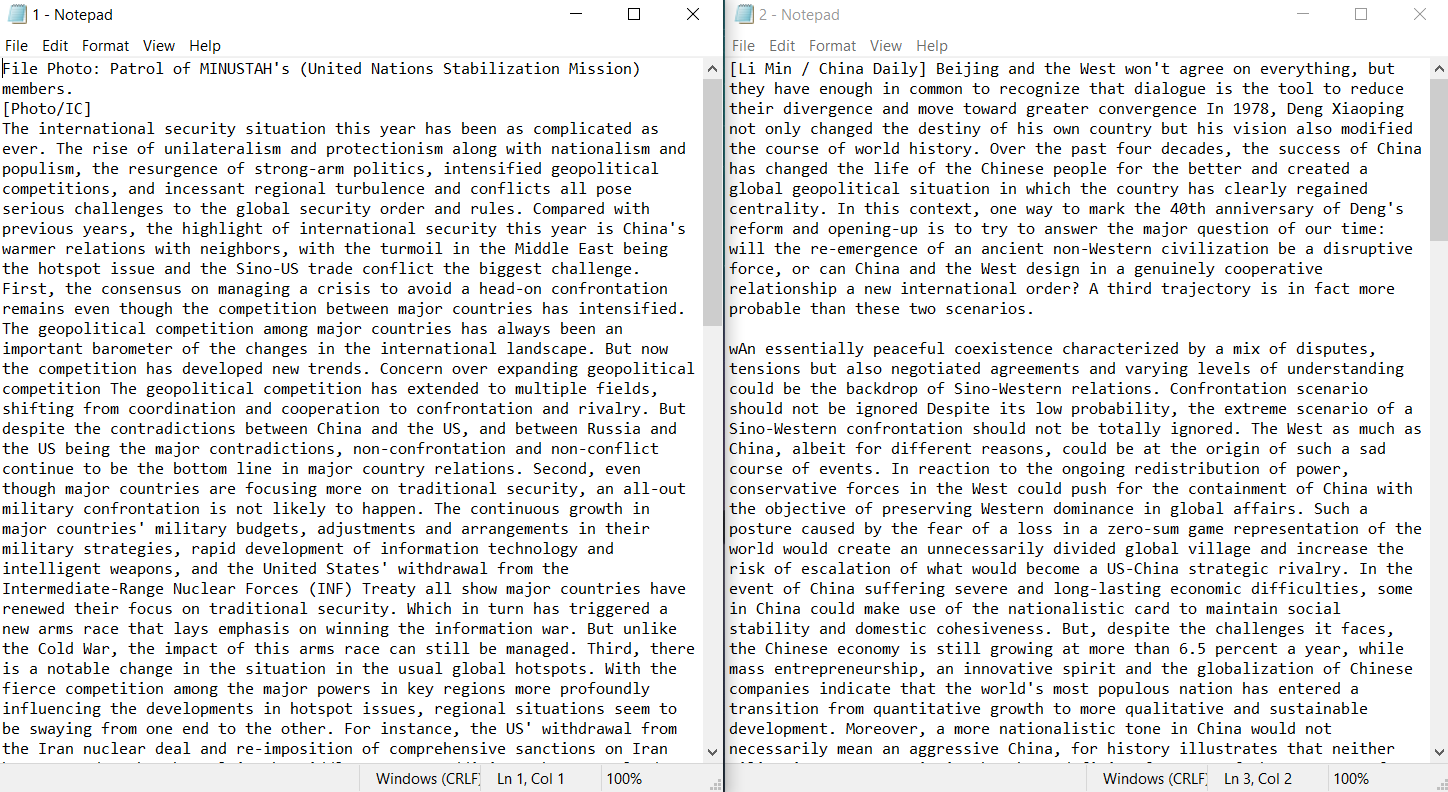
\includegraphics[width=1.0\linewidth]{diagram/chinaNews}}
	\caption{Sample of news article form China}
	\label{fig:chinanews}
\end{figure}
\vspace{-1cm}
To clean the data set, this study will used WebAnno annotation tool to manually annotate keywords based on corresponding entities. After that, stemming process will be taken to reduce verb into its basic form. Finally, these corresponding entity based on different word characteristics are grouped them into 5 tuple of <Actor, Action, Object, Location, Object>. 


\section{Performance Measurement}
To measure the performance of the prediction model, precision and recall as well as F1-score are used. Confusion matrix in Figure 3.4 also provides classification of evaluation between actual event and predicted event.

\begin{figure}[H]
	\centering
	\fbox{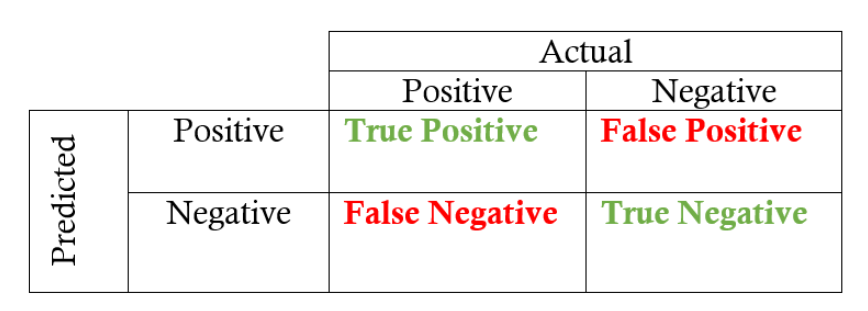
\includegraphics[width=0.7\linewidth]{diagram/confusionMatrix}}
	\caption{Confusion Matrix}
	\label{fig:confusionmatrix}
\end{figure}
\vspace{-1cm}

Precision is the percentage of relevant results while recall is the percentage of total relevant result that correctly identify from prediction model. Both formula of precision and recall are
\begin{equation}\label{3.3}
\textbf{Precision} = \frac{True Positive}{Actual Results} 
\end{equation}
\begin{equation}\label{3.4}
\textbf{Recall} = \frac{True Positive}{Predicted Results} 
\end{equation}
To summarise the usage of precision and recall, F1 score is used to give a higher priority to maximizing precision and recall to the prediction model. F1 score is formulated from 
\begin{equation}\label{3.5}
\textbf{F1 score} = 2 * \frac{Precision * Recall}{Precision + Recall} 
\end{equation}

\section{PSM 1 Gantt Chart}
The PSM 1 Gantt Chart is in Appendix A. 

\section{Summary}
Chapter 3 discussed the method and steps to use throughout the project. In Research Framework, each of the phase will generate important output and consecutively become input for the next phases. For phase 1, data corpus is built from unstructure textual data from SCS-related news article and represent in 5 tuple format. Then, in phase 2, the sanitised event are generalised and an abstraction tree is built by using HAC hierarchical clustering. Causality prediction rules is also generated in order to generate predicted effect events. Finally, in phase 3, prediction model is trained and the output is filtered in order to produce high quality and reliability output. The prediction model is then evaluate by performance measurement such s precision and recall. Data set used in this study are also stated as it is the main source for this project.  


%Chapter 4
\chapter{Experimental Setup}
\section{Introduction}
In this chapter, an experimental setup is done by working on phase 1 in the Research Framework. Steps in Phase 1 such as data collection, text preprocessing and event representation will be explained in details. After that, this chapter displays the initial result and finding of phase 1. Finally, the chapter ends with a summary of the chapter.

\section{Text Preprocessing and Event Extraction}
In phase 1, the data is collected from online news article that is related to South China Sea conflict with the selected keywords. In order to present the process of text preprocessing, sample sentence is taken from one of the news article. The sample of sentences is \textit{"Two years after the arbitration court ruling in favour of Philippines’ South China Sea case and rejecting China’s so-called nine-dash line, disputes continue to rage even as China and ASEAN formally enter negotiations towards a Code of Conduct framework."}, taken from VietnamNews. In this sentence, we can obtain that the SCS disputes continue to rise as issues occur in SCS countries.

In phase 1, text preprocessing will be the primary work. Purpose of text preprocessing is to structure the unstructured textual data and extract useful information while ignoring those duplicated and meaningless words. There are few steps involved in text preprocessing such as annotation, stemming and representation. Figure 4.1 shows the flow of text preprocessing in phase 1.
\begin{figure}[H]
	\centering
	\fbox{\includegraphics[width=0.8\linewidth]{"diagram/phase1 steps"}}
	\caption{Flow of Text Preprocessing}
	\label{fig:phase1-steps}
\end{figure}
\vspace{-1cm}

At the beginning of the project, this project tend to extract information by using standard Named Entity Recognisation (NER). NER is a part of information extraction that identify named entity within a sentence.  However, standard NER has its limitation that only able to recognise person, organisation, location and time. Figure 4.2 shows the limitation of NER extraction by using sample sentence. 
\begin{figure}[H]
	\centering
	\fbox{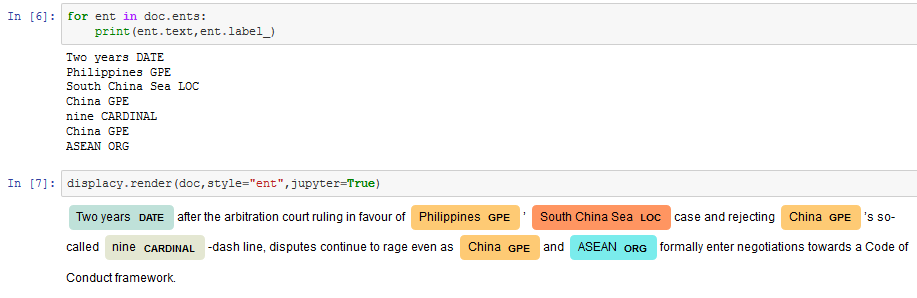
\includegraphics[width=1.0\linewidth]{diagram/spacy4}}
	\caption{Limitation of standard NER for only extracting person, organisation, location and time}
	\label{fig:spacy4}
\end{figure}
\vspace{-1cm}

Thus, manual annotation is used to annotate important entity such as action, object and instrument. For annotation, WebAnno annotation tool is used. WebAnno is a general purpose web-based linguistic annotation tool including various layers of morphological, syntactical and semantic annotations. By using WebAnno, this study is able to add custom entity and annotate them with matched words. Figure 4.3 shows annotation of sample sentence in WebAnno. 
   
\begin{figure}[H]
	\centering
	\fbox{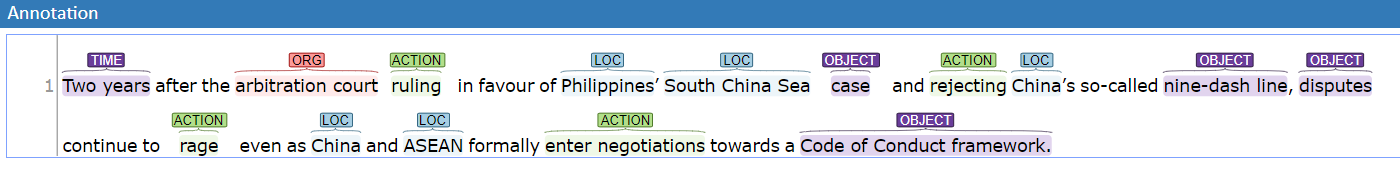
\includegraphics[width=1.0\linewidth]{diagram/annotation}}
	\caption{Annotation of sample sentence in WebAnno}
	\label{fig:annotation}
\end{figure}
\vspace{-1cm}
After annotation, the output is printed using CoNLL-2002 format. CoNLL-2002 format is a data output format which consists of two columns separated by a single space. There are 2 attributes in CoNLL-2002. The first one is tag format which B denotes first item and I denotes non-initial words. The second one is the entity tag of the words. Figure 4.4 shows the CoNLL-2002 data output of annotation. In this format, the custom entity such as \textit{TIME}, \textit{ACTION} and \textit{OBJECT} will be defined accordingly. 
\begin{figure}[H]
	\centering
	\fbox{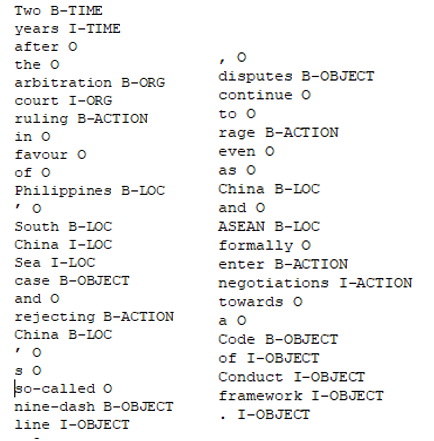
\includegraphics[width=0.9\linewidth]{diagram/annotationResult}}
	\caption{Annotation in CoNLL-2002 format}
	\label{fig:annotationresult}
\end{figure}
\vspace{-1cm}

After that, all the entity tag with \textit{ACTION} will be normalised through stemming. Stemming is the process where convert verb into its basic form. For example, in the sample sentence, "ruling" and "rejecting" are the entity tag with \textit{ACTION}. After stemming, they will become "rule" and "reject" respectively. In the following steps, these custom entity will be assigned into 5 tuple of <Actor, Action, Object, Location, Timestamp> for event representation. Both stemming and representation will be done in the future.  


\section{Summary}
In this chapter, the preliminary works in phase 1 is done on the data collected from South China conflict.First, the annotation model is preset with custom entity tag because there are limitation of entity in standard NER. The limited entity in standard NER are person, organistion, location and time which are required to have more in this study. Then, the annotation is then output as CoNLL-2002 format as it provides simple yet essential output for the further text processing. After that, the words with custom entity of \textit{ACTION} are stemmed into its basic form. Finally, these customer NER will be represented in 5 tuple approach. These preliminary works is important so that the following text processing will be successful and works on the right path.  

%Chapter 5
\chapter{Conclusion}
\section{Conclusion Remarks}
After performing preliminary task in previous chapter, the initial result had been partially achieved. Data source is cleaned and sanitised.  Cleaned data is suitable for further processing to obtain valuable information. However, there are a lot of works needs to be done in order to reach the stage of building up prediction model and it will be discussed in the next section. In this study, the main attributes is causality. Causality is used to indicate the relation between cause and effect. In the future works, this study needs to extract the causality from news article and compare with world ontology to get precise knowledge on the same domain. Besides, Pundit algorithm needs to be followed from step to step as a guideline in this study. Pundit algorithm provides a prediction framework that start from learning the causality of events until the prediction of future event. By obeying Pundit algorithm, the predicted effect event will have high reliability and precision. 

\section{Future Works}
After annotating entity from sample sentence in previous chapter, these entities need to be assigned based on their characteristic which manually defined by researcher. In addition, another challenge is to put all these entities into corresponding tuple <Actor, Action, Object, Location, Timestamp>. This step might require some recursive algorithm that constantly load matched entity into the tuple.

In the next phase, which is phase 2, the extracted tuples are being generalised in order to reduce the size of corpus. Generalisation is measured by using the similarity of the event pairs based on world ontology. By generalising the event pairs, multiple generalisation path will be created and the shortest path are defined as minimal generalisation path. With minimal generalisation path, an abstraction tree is built and the nodes within the abstraction tree is cluster through HAC hierarchical clustering. After that, causality prediction rules is set in the form of <Pattern, Constraints, Priority> for the preparation of input cause event to generate most possible effect event. 

In phase 3, the prediction model based on abstraction tree is built. Test data are taken from new input cause event and the new event will propagate throughout the abstraction tree to find the matched node. During the propagation, minimal generalisation path and causality prediction rules are used to guide the input events for the desired effect event. To maximize the performance of prediction model, filtering process will take place to eliminate inappropriate predicted effect event. Filtering process will be handled by PMCI calculation to match up the relativeness between cause and effect. Finally, performance measure by using precision and recall will be evaluated the accuracy and precision of the prediction model. 

\section{Summary}
This chapter discusses the overall conclusion and the future works that require completing within this project. After finishing the steps in previous chapter, there are still a lot of works need to be done, such as event generalisation, causality prediction rules generation, building up an abstraction tree, etc. Future work will be done on the following chapter and causality will be focus in this study so that event pairs has strong causal relation that satisfy the requirement of event prediction.  



\bibliographystyle{utmthesis-authordate}
\bibliography{reference}

\appendix
\chapter{PSM Gantt Chart}
\begin{figure}[H]
	\centering
	\includegraphics[angle=90,width=1.0\linewidth]{"diagram/Thesis Gantt Chart NEW"}
	\label{fig:thesis-gantt-chart-new}
\end{figure}


\endmatter
\end{document}
